

\chapter{Результаты экспериментов} \label{AppendixB}

\vspace{-1cm}
\begin{figure}[h]
\centering
\includegraphics[scale=0.9]{Pictures/pic_firstTimeUntilServ_stationar.png} 
\caption{Динамика среднего времени ожидания произвольного требования потока $\Pi_1$. Система со стационарным режимом}
\label{Experiment:timeUntilServiceFirst:stationar}
\end{figure}

\begin{figure}[h]
\centering
\includegraphics[scale=0.9]{Pictures/pic_secondTimeUntilServ_stationar.png} 
\caption{Динамика среднего времени ожидания произвольного требования потока $\Pi_3$. Система со стационарным режимом}
\label{Experiment:timeUntilServiceSecond:stationar}
\end{figure}

\begin{figure}[h]
\centering
\includegraphics[scale=0.9]{Dissertation/Work_structured/Pictures/pic_inputOutputFirstFlow_stationar.png}
\caption{Динамика среднего числа поступивших и ушедших требований потока $\Pi_1$  за единицу времени. Система со стационарным режимом}
\label{Experiment:inputOutputFirstFlow:stationar}
\end{figure}

\begin{figure}[h]
\centering
\includegraphics[scale=1]{Dissertation/Work_structured/Pictures/pic_inputOutputSecondFlow_stationar.png}
\caption{Динамика среднего числа поступивших и ушедших требований потока $\Pi_3$ за единицу времени. Система со стационарным режимом}
\label{Experiment:inputOutputSecondFlow:stationar}
\end{figure}

\begin{figure}[h]
\centering
\includegraphics[scale=1]{Dissertation/Work_structured/Pictures/pic_firstTimeUntilServ.png}
\caption{Динамика среднего времени ожидания произвольного требования потока $\Pi_1$. Система без стационарного режима}
\label{Experiment:timeUntilServiceSecond:nonstationar}
\end{figure}

\begin{figure}[h]
\centering
\includegraphics[scale=1]{Dissertation/Work_structured/Pictures/pic_inputOutputFirstFlow.png}
\caption{Динамика среднего числа поступивших и ушедших требований потока $\Pi_3$ за единицу времени. Система со стационарным режимом}
\label{Experiment:inputOutputFirstFlow}
\end{figure}


%0_1_thres_10_target
\begin{figure}[h]
\centering
\includegraphics[scale=0.85]{Pictures/0_1_thres_10_target_fact.png} 
\caption{Области стационарности системы. $\lambda_3=0.1$, $L=10$}
\label{Experiment:stationar}
\end{figure}
\begin{figure}[h]
\centering
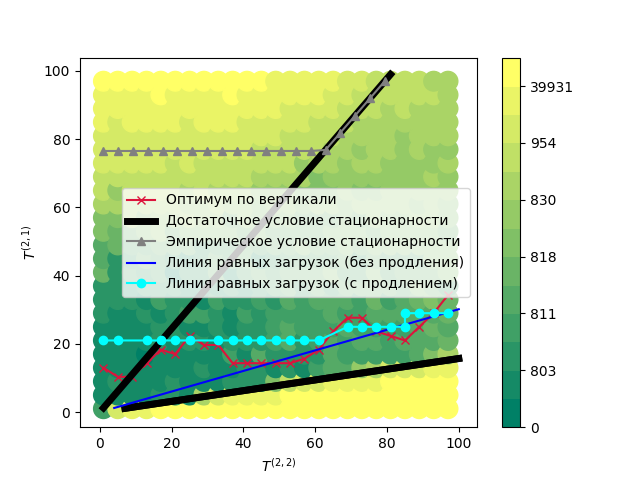
\includegraphics[scale=0.9]{Pictures/0_1_thres_10_target_new.png} 
\caption{Поиск оптимальных параметров системы}
\label{Experiment:targets}
\end{figure}




\begin{figure}
\begin{multicols}{2}
    \includegraphics[width=1.15\linewidth]{Pictures/0_1_thres_-1_fact.png}\par 
    \includegraphics[width=1.15\linewidth]{Pictures/0_1_thres_5_fact.png}\par 
    \end{multicols}
\begin{multicols}{2}
    \includegraphics[width=1.15\linewidth]{Pictures/0_1_thres_10_fact.png}\par
    \includegraphics[width=1.15\linewidth]{Pictures/0_1_thres_15_fact.png}\par
\end{multicols}
\caption{Области стационарности для разных значений $L$. Слева-направо, сверху-вниз $L=-1$; $5$; $10$; $15$}
\label{different:thres}
\end{figure}

\vspace{-10cm}
\begin{figure}[H]
\begin{multicols}{2}
    \includegraphics[width=1.2\linewidth]{Pictures/0_1_thres_10_fact.png}\par 
    \includegraphics[width=1.2\linewidth]{Pictures/0_2_thres_10_fact.png}\par 
    \end{multicols}
\caption{Области стационарности для разных значений $\lambda_1$. Слева $\lambda_1=0.1$, справа $\lambda_1=0.2$}
\label{Experiment:intensities}
\end{figure}
